\documentclass[]{scrartcl}

%Packages________________
\usepackage[normalem]{ulem}
\usepackage{cancel, xcolor}
\usepackage{parskip}
\usepackage{caption, subcaption}
\usepackage[Spanish,es-tabla,es-noshorthands]{babel}
\usepackage{newtxtext}
\usepackage[varvw]{newtxmath}
\usepackage{booktabs, colortbl, bigstrut, multirow, multicol}
\usepackage{url}
\usepackage{pgfplots}
\usepackage{graphicx}
\usepackage{amsmath}
\usepackage{tabularx}
\usepackage{floatrow}
\usepackage{float}
\usepackage{cancel}
\usepackage[spanish]{cleveref}
\usepackage{tikz}
\usetikzlibrary{arrows.meta}
\crefname{table}{tabla}{tablas}
\usepackage{wrapfig}
\usepackage{adjustbox}
\usepackage{geometry}
\usepackage{lipsum}
\usepackage{fancybox}
\geometry{
	top=2.4cm,
	bottom=2.4cm,
	left=2.3cm,
	right=2.3cm
}

\usepackage[
    backend=biber,
	citestyle=verbose-ibid,
    bibstyle=authoryear-icomp,
    natbib=true,
    url=true, 
    doi=true,
    eprint=false
]{biblatex}

\addbibresource{ref.bib}

%Commands________________
\newcommand\hcancel[2][black]{\setbox0=\hbox{$#2$}%strikeout
\rlap{\raisebox{.45\ht0}{\textcolor{#1}{\rule{\wd0}{1pt}}}}#2} 

\renewcommand\theequation{\Alph{equation}}

\DeclareMathOperator\Log{Log}
\DeclareMathOperator\Ln{Ln}


%\renewcommand\thesubsection{\Alph{subsection}}

%Titlepage_________________
\title{\vspace{-1.8cm} Práctica de Simulación - Parte 1}
\author{Álvaro Jerónimo Sánchez}
\date{}

%Document_____________
\begin{document}
\maketitle
\setcounter{section}{0}
\renewcommand{\tablename}{Tabla}

\section{Práctica 1: Análisis de circuitos en cc}

\subsection{Ejercicio 1}

\begin{wrapfigure}{r}{0.6\textwidth}
\centering
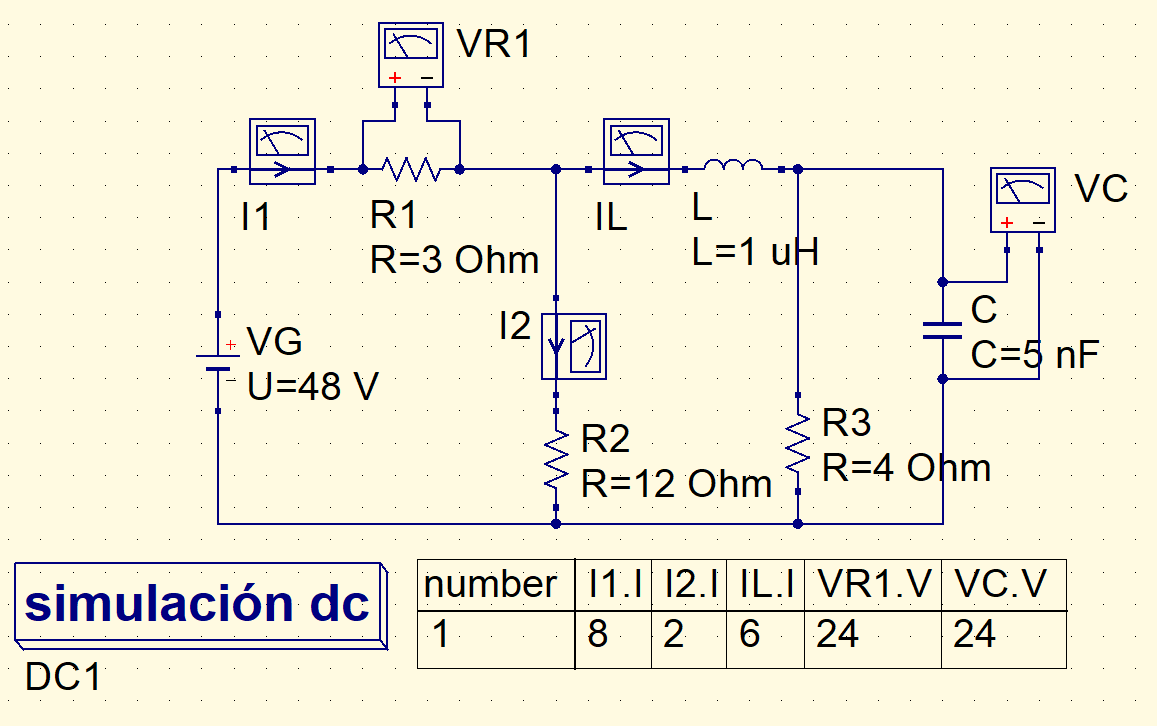
\includegraphics[width=0.9\columnwidth]{../1-1.png}
\end{wrapfigure}

Este se trata de un circuito simple con tres mallas y ninguna fuente dependiente. 

El condensador aún no se ha estudiado en el tema, por lo que la medida del voltaje $V_C$ se ha sacado directamente de la simulación en \textit{Qucs}: $\boxed{V_C=24\; V}$. La bobina es ideal y la corriente en ésta no depende del tiempo, por lo que su  voltaje será $V_L=0$. Teniendo esto en cuenta, planteamos las ecuaciones de las mallas \textit{1, 2 y 3} (de izquierda a derecha) y sustituimos valores para hallar $V_{R1}$: \\ \vspace{-8pt}

\begin{minipage}{.4\textwidth}
\begin{gather*}
	\left\{
	\begin{array}{l}
		(1)\; V_G=V_{R1}+V_{R2}\\
		(2)\; 0=V_{R2}+\cancel{V_L}+V_{R3}\\
		(3)\; 0=V_{R3}+
	\end{array}
	\right. \\
	\rightarrow V_{R2}=-V_{R3}=V_C\\
	V_{R1}=V_G-V_C \Rightarrow \boxed{V_{R1}=24\; V}
\end{gather*}
	\end{minipage}
	\hfill\vline\hfill
	\begin{minipage}{.4\textwidth}
Para hallar la intensidad $I_1$ e $I_2$, simplemente aplicamos la Ley de Ohm:
\begin{gather*}
I_1=\frac{V_{R1}}{R_1}\Rightarrow \boxed{I_1=8\; A}\\
I_2=\frac{V_C}{R_2}\Rightarrow \boxed{I_2=2\; A}
\end{gather*}
\vspace{2pt}
\end{minipage}
\hrule

Para obtener $I_L$, emplearemos el método de nodos (\textit{Primera Ley de Kirchoff}):
\begin{gather*}
	I_1-I_2-I_L=0\Rightarrow I_L=I_1-I_2\Rightarrow \boxed{I_L=6\; A}
\end{gather*}

\subsection{Ejercicio 2}

\begin{wrapfigure}{r}{0.6\textwidth}
\centering
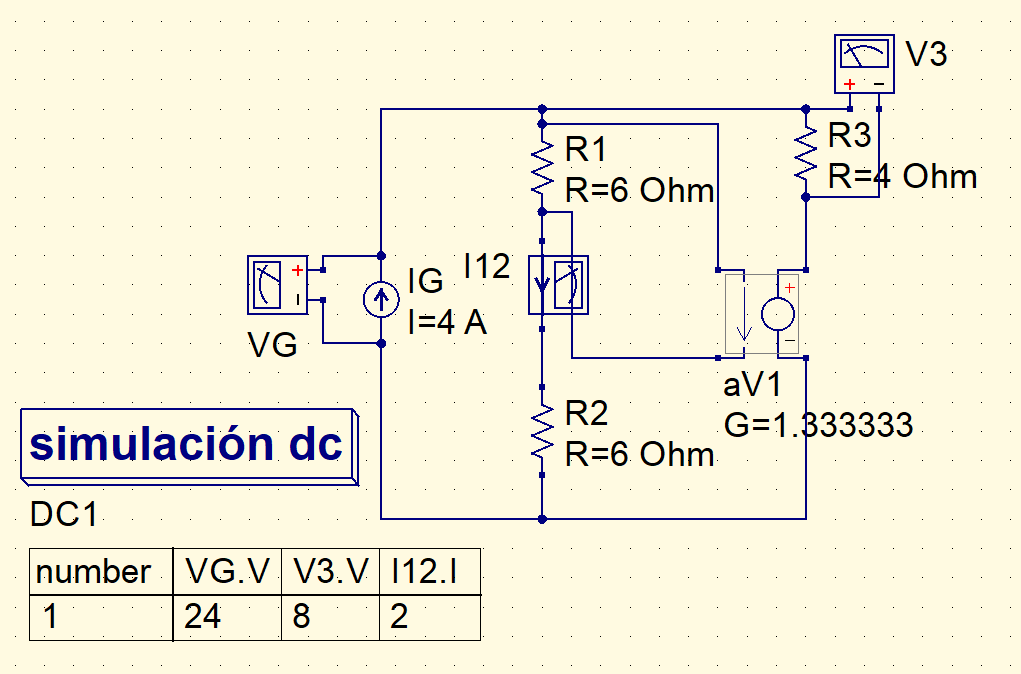
\includegraphics[width=0.9\columnwidth]{../1-2.png}
\end{wrapfigure}

En este circuito se incluye una fuente de tensión dependiente del voltaje $V_{R1}$ con una $a=\frac{4}{3}$, por lo que $aV_1=\frac{4}{3}V_{R1}$. Ya que en serie la corriente es constante, $I_{R1}=I_{R2}=I{12}$, y al ser $R_1=R_2=6\; \Omega$, los voltajes de ambas resistencias serán iguales, aplicando la Ley de Ohm: $V_{R1}=V_{R2}$. 

Las ecuaciones de las mallas son:
\begin{gather*}
	\left\{
	\begin{array}{l}
		(1)\; V_G=2V_{R1}\\
		(2)\; \frac{4}{3}V_{R1}=2V_{R1}+V_{R3}
	\end{array}
	\right.
\end{gather*}

\clearpage 
Aplicando la Ley de Ohm, en la rama central tenemos que la intensidad es $I_{12}=\frac{V_{R1}}{R_1}$, y en la derecha será $I_3=\frac{-V_{R3}}{3R_3}=\frac{2V_{R1}}{R_3}$. Aplicando la ley de nodos, tenemos que:
\begin{gather*}
	I_G=I_{12}+I_{3}=V_{R1}\left( \frac{1}{R_1}+\frac{2}{3R_3} \right) \Rightarrow V_{R1}=12\; V\\
	\rightarrow V_G=2V_{R1}=\boxed{24\, V}\; ; \; I_{12}=\frac{V_G}{2R_1}=\boxed{2\, A} \; ; \; V_{R3}=\frac{2}{3}V_{R1}=\frac{V_G}{3}=\boxed{8\, V}
\end{gather*}

\subsection{Ejercicio 3}

\begin{wrapfigure}{r}{0.6\textwidth}
\centering
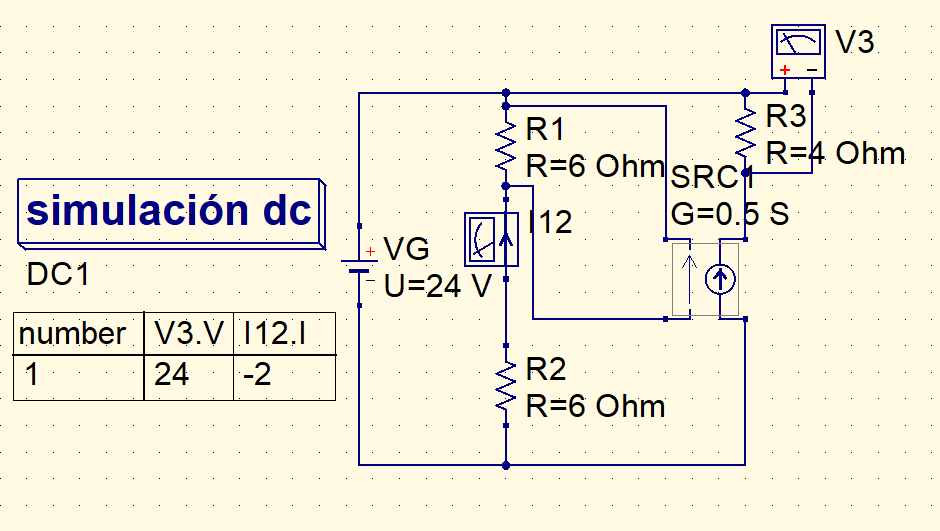
\includegraphics[width=0.9\columnwidth]{../1-3}
\end{wrapfigure}

Este circuito es muy similar al anterior, diferenciándose en que ahora la fuente dependiente del voltaje $V_R1$ proporciona corriente, con una $g=0.5\, S$; y además la fuente de la rama izquierda es de voltaje, proporcionando $V_G=24\, V$. Las resistencias están dispuestas de la misma manera, pero la intensidad $I_12$ que nos piden calcular esta vez está dirigida hacia arriba, por lo que tendrá signo contrario.

Al tener $g=0.5\, S$, la intensidad de la fuente dependiente será $I_G=0.5V_{R1}$. Aplicando la ecuación para la malla 1 (izquierda), podemos hallar $V_{R1}$, y con ello también $I_G$ que será igual que $I_{R3}$, ya que ambos componentes están en serie.
\begin{gather*}
	(1)\; V_G=2V_{R1} \rightarrow V_{R1}=12\, V \\
	I_G=I_{R3}=0.5V_{R1}=6\, A
\end{gather*}

Tras esto, podemos hallar $I_{12}$ y $V_{R3}$ simplemente aplicando la Ley de Ohm, teniendo en cuenta de que $I_{12}$ se encuentra ahora en el sentido contrario:
\begin{gather*}
	V_{R3}=I_{R3}R_3 =\boxed{24\, V} \; ; \; I_{12}=\frac{-V_{R1}}{R_1} =\boxed{-2\, A}
\end{gather*}

\subsection{Ejercicio 4}

\begin{wrapfigure}{r}{0.6\textwidth}
\centering
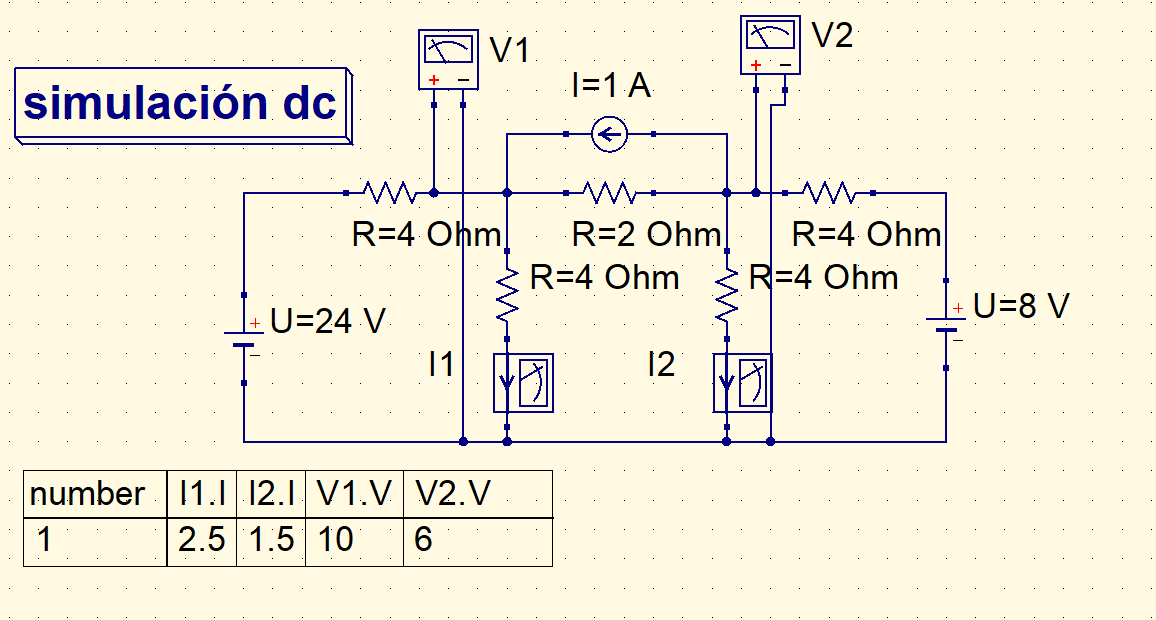
\includegraphics[width=0.9\columnwidth]{../1-4}
\end{wrapfigure}

Este circuito consta de cuatro mallas distintas, mayoritariamente formadas por resistencias, y con dos fuentes de voltaje y una de corriente, todas independientes.

Planteamos la ley de los nodos para el nodo 1 y en el nodo 2 para posteriormente relacionarlas y hallar $V_1$ y $V_2$, teniendo en cuenta que el cable inferior es el de referencia: \clearpage
\begin{gather*}
	(1)\; I_G=I_{R1}+I_1+I_{R3} \rightarrow 0=\frac{V_1-24}{R_1}+\frac{V_1-0}{R_2}+\frac{V_1-V_2}{R_3} -1\\
	\Rightarrow 2V_1-V_2-14=0\\
	(2)\; 0=I_G+I_{R3}+I_2+I_{R5} \rightarrow 0=1+\frac{V_2-V_1}{R_3}+\frac{V_2-0}{R_4}+\frac{V_2-8}{R_5}\\
	\Rightarrow -2V_1+4V_2-4=0
\end{gather*}

Sustituyendo hallamos que: $\boxed{V_1=10\, V}\; ; \; \boxed{V_2=6\, V}$. Con esto podemos hallar las intensidades con una aplicación directa de la Ley de Ohm:
\begin{gather*}
	I_1=\frac{V_1}{R_2}=\boxed{2.5\, A} \; ; \; I_2=\frac{V_2}{R_4}=\boxed{1.5\, A}
\end{gather*}

\subsection{Ejercicio 5}

\begin{wrapfigure}{r}{0.6\textwidth}
\centering
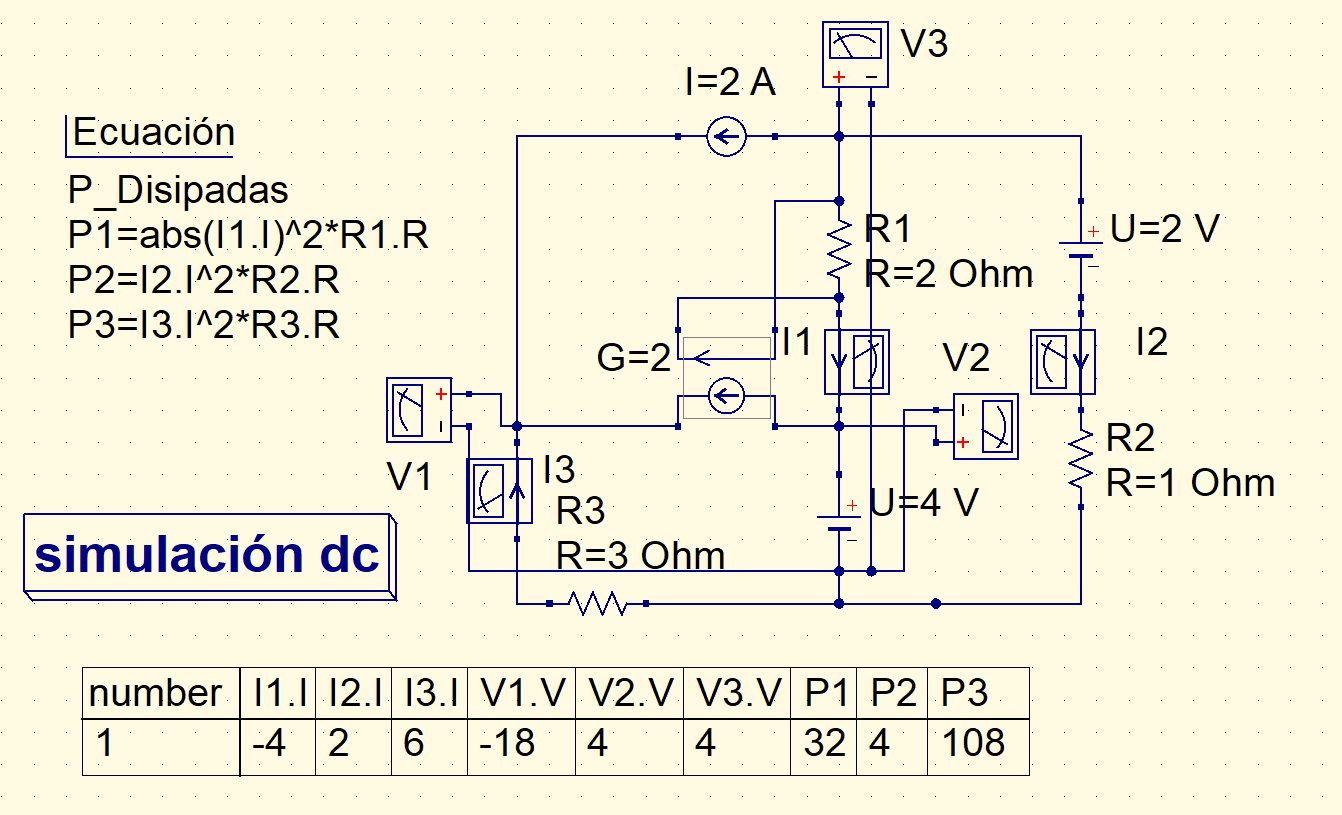
\includegraphics[width=0.9\columnwidth]{../1-5.png}
\end{wrapfigure}

Este circuito es más complejo, conteniendo dos fuentes de tensión y dos de corriente, una de éstas dependiente de la intensidad $I_1$ y proporcionando $I_D=2I_1$. Se ha tomado como referencia el nodo inferior derecho, y se ha tenido problemas a la hora de hallar las potencias disipadas inicialmente, ya que algunas aparecían en forma compleja. Esto se debía a una intensidad negativa (signo contrario al del sentido en el que se ha medido), por lo que se ha solucionado con un valor absoluto. 

No se ha conseguido llegar a todos los valores numéricos de forma demostrada a mano, pero las ecuaciones de los nodos y mallas son las siguientes:

\vspace{10pt}
\begin{minipage}{.4\textwidth}
	\textbf{Nodos:}
	\begin{gather*} \left\{
		\begin{array}{l}
			(1)\; I_D+I_G=I_{R3} \Rightarrow 2I_1+2=I_{R3}\\
			(2)\; I_1=I_D+I_{V_{G1}} \Rightarrow I_{V_{G1}}=-I_1\\
			(3)\; 0=I_G+I_1+I_{V_{G2}} =2+I_1=I_{R2}
		\end{array}
		\right. 
	\end{gather*}
	\vspace{7pt}
\end{minipage}
\hfill\vline\hfill
\begin{minipage}{.4\textwidth}
	\textbf{Mallas:}
	\begin{gather*} \left\{
		\begin{array}{l}
			(1)\; 0=V_{IG}+V_{ID}+V_{R1}\\
			(2)\; V_{G1}=V_{ID}+V_{R3}\\
			(3)\; V_{G1} + V_G2=V_R1+\cancel{V_{R2}}
		\end{array}
		\right.\\
		\Rightarrow V_{R1}=6\, V
	\end{gather*}
\vspace{2pt}
\end{minipage}
\hrule

\clearpage

\section{Práctica 2:}

\subsection{Ejercicio 1}

\begin{figure}[h]
\centering
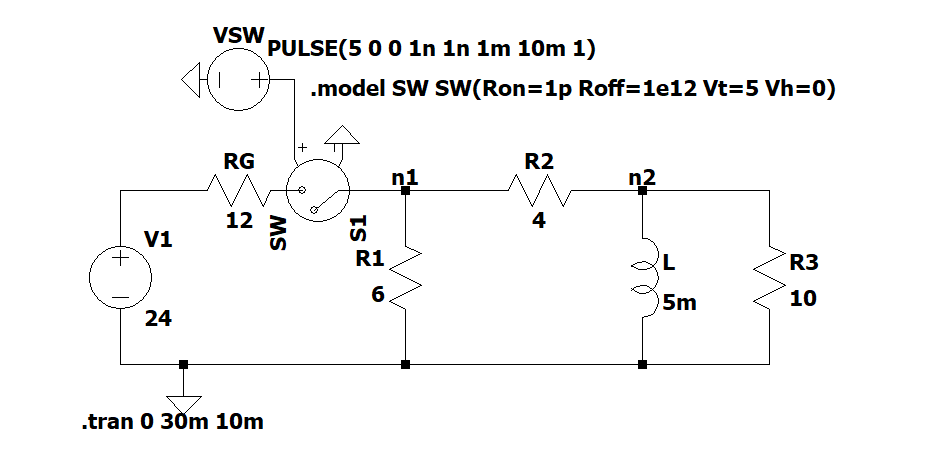
\includegraphics[width=0.8\columnwidth]{../2-1.png}
\end{figure}

\begin{wrapfigure}{r}{0.6\textwidth}
\centering
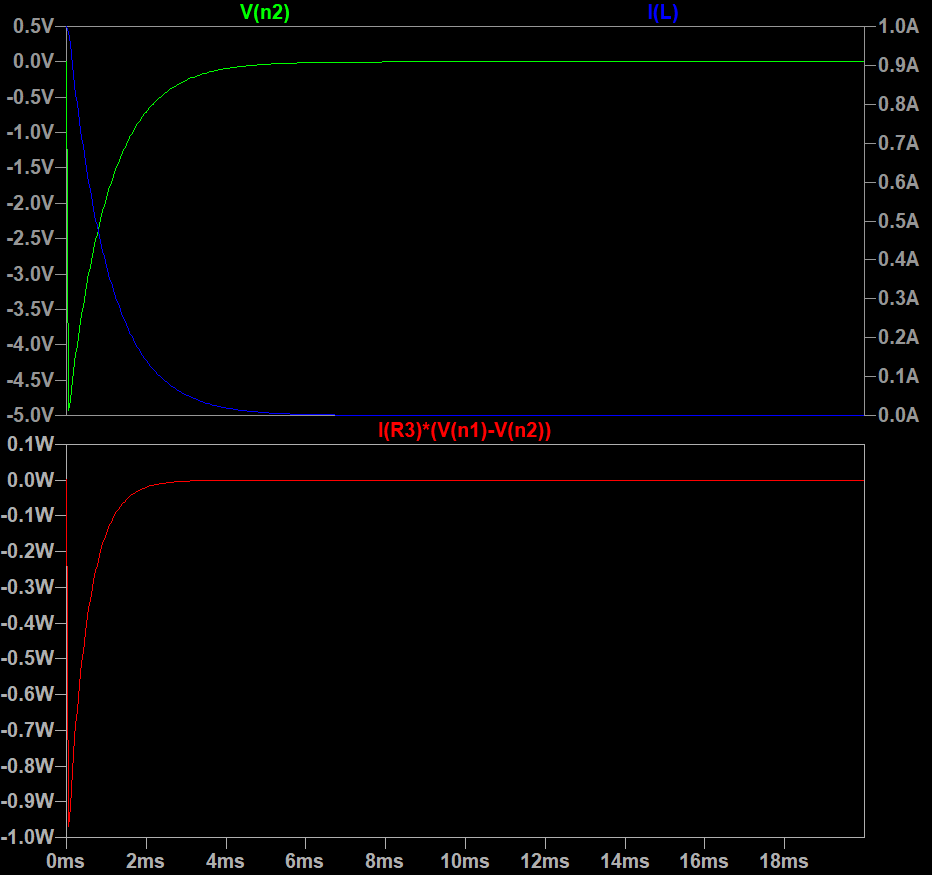
\includegraphics[width=0.9\columnwidth]{../2-1g.png}
\end{wrapfigure}

Para las siguientes secciones de este documento se ha usado \textit{LTspice} para realizar las simulaciones. El componente \textit{"SW"} se trata de un interruptor activado por voltaje, que es el único tipo que LTspice ofrece. Se ha elegido que este se cerrará mientras reciba un voltaje de 5 V. Se ha conectado a una fuente de 5 V que primeramente emite un pulso que dura 10 ms, para que se cargue la bobina, y tras esto deja de emitir, lo que causa que el interruptor se abra. Se ha empezado a recoger datos tras los 10ms, para simplemente ver las condiciones iniciales de un circuito con una bobina cargada que se abre en t=0 y graficar a partir de ahí.

En este ejercicio hay una bobina, por lo que las intensidades y voltajes variarán con el tiempo. Al abrirse el interruptor, la primera malla queda desconectada, por lo que la fuente ya no suministra voltaje y la resistencia $R_G$ ya no tiene influencia. Tras hacer el circuito equivalente por asociación de resistencias, hallamos que $\frac{1}{R_{EQ}}=\frac{1}{R_1+R_2}+\frac{1}{R_3}=5\, \Omega$. Las dos ramas de la derecha tienen la misma resistencia total ($10\, \Omega$), por lo que sabemos que la intensidad de cada rama será $I_{rama}=\frac{I_{Tot}}{2}$.

Para hallar el voltaje $v_2$ que pasa por la resistencia $R_2$ aplicamos la ley de Ohm teniendo en cuenta que se encuentra en función de una $i_L(t)$. Sabiendo que la solución estacionaria ($A$) para la intensidad es 0, ya que la fuente no está conectada, podemos hallar la condición inicial sustituyendo $t=0$, por lo que tenemos los parámetros necesarios para hallar $i_L(t)$ y $v_2(t)$:
\begin{gather*}
	v_2(t)=\frac{i_L(t)}{2}R_2=2i_L(t)\; ; \; i_L(0)=Be^0=1\, A\\
	\Rightarrow \boxed{i_L(t)=e^{-\frac{t}{\tau}}}\; \boxed{v_2(t)=2e^{-\frac{t}{\tau}}}
\end{gather*}

Para tiempos $t>0$, $\tau=\frac{L}{R}=10^{-6}\, s$, por lo que hallamos la potencia disipada en $R_3$ con:
\begin{gather*}
	P_{R3}(t)=\left( \frac{i_l(t)}{2} \right)^2 R_3 = \boxed{2.5e^{-2t\cdot 10^{-6}}\, W}
\end{gather*}

\subsection{Ejercicio 2}

\begin{figure}[h]
\centering
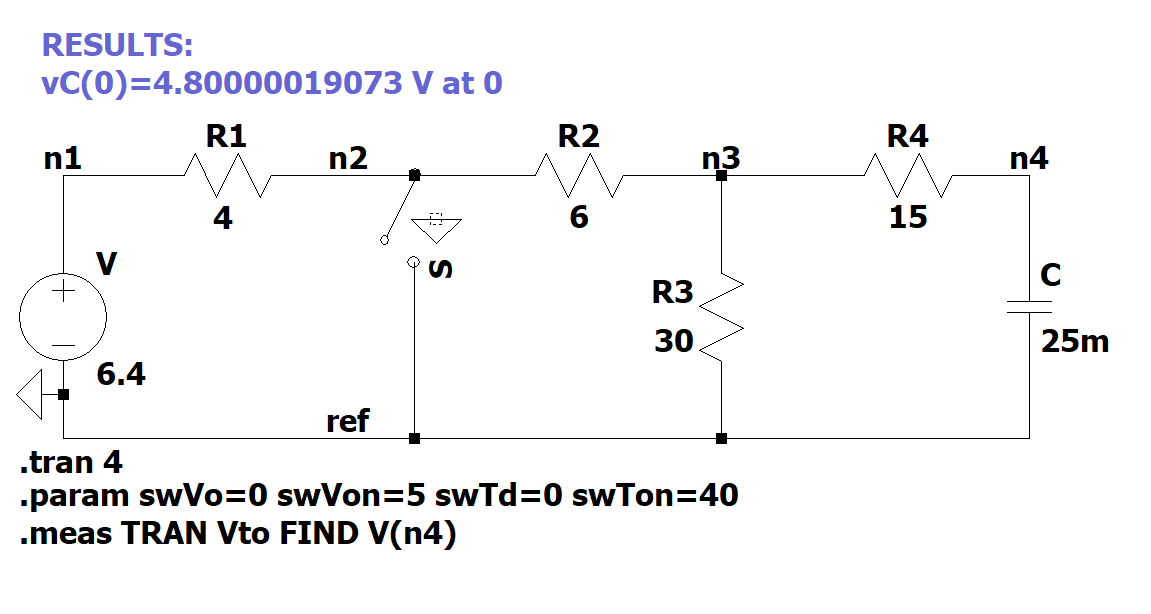
\includegraphics[width=0.6\columnwidth]{../2-2.png}
\end{figure}

\begin{wrapfigure}{r}{0.6\textwidth}
\centering
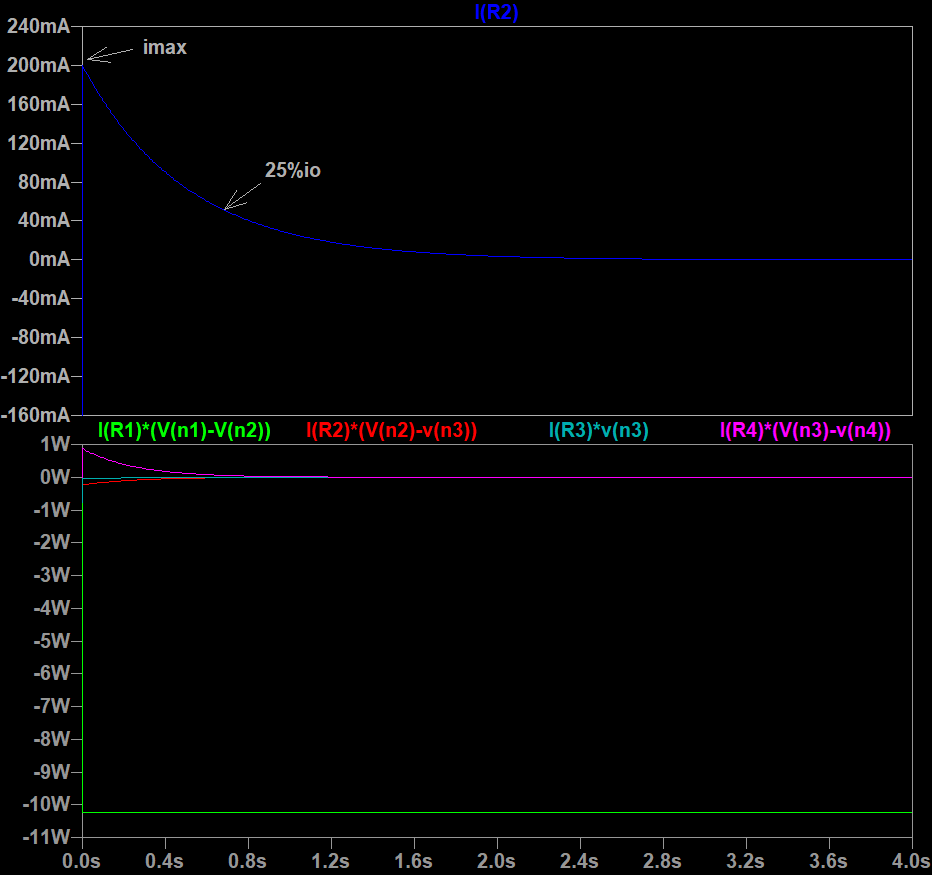
\includegraphics[width=0.9\columnwidth]{../2-2g.png}
\end{wrapfigure}

Cabe mencionar que la clase de interruptores del ejercicio anterior se representarán desde ahora con un subcircuito para mejor claridad visual. Éste se puede encontrar adjunto en el apéndice (\cref{fig:sw}) con la explicación de cada parámetro. Se ha asumido que los valores de las resistencias son en Ohmios, aunque en el esquema se dan en $W$, pero posiblemente sea una errata, ya que si no, sería imposible de simular y resolver.

En $t\rightarrow\infty$ el condensador se ha descargado, por lo que la solución estática ($A$) para el voltaje es cero. En $t<0$ el condensador está lleno, lo que actúa como una rama abierta, desconectando $R_4$ del resto del circuito. En cambio, para $t>0$ la batería se cortocircuita, aislando $R_1$. Teniendo esto en cuenta, procedemos a hallar las resistencias equivalentes en cada caso y el parámetro $\tau$ para hallar la expresión del voltaje en función del tiempo. Antes de esto, debemos hallar el voltaje inicial ($v_C(0))$, que será la diferencia entre el nodo 4 y tierra, ya que $R_4$ está desconectada:
\begin{gather*}
	v_C(0)=I_0R_{eq_o} = \frac{6.4}{4+6+30}\cdot R_3 = \boxed{4.8\, V}\\
	v_C(t)=0+Be^{-\frac{t}{CR_{eq}}}\xrightarrow[\left(R_{eq}=\frac{1}{\frac{1}{6}+\frac{1}{30}}+15\right)]{} \boxed{v_C(t)=4.8e^{-2t}} 
\end{gather*}

Con esto, podemos hallar la $i(t)$ de la resistencia de $r\,\Omega$ aplicando Ohm tras hallar el voltaje que pasa por ésta, que será $V(n3)-\cancelto{0}{n2}$, ya que el nodo 2 está conectado a tierra. Aplicando mallas tenemos que:
\begin{gather*}
	0=I_{R2}+I_{R3}+I_{R4}=\frac{V_{n3}-0}{6}+\frac{V_{n3}-0}{30}+\frac{V_{n3}-V_C}{15}=8V_{n3}-2V_C\\
	V_{n3}=\frac{V_C}{4}\\
	i(t)=\frac{V_C}{4R_2}=\boxed{0.2e^{-2t}} \rightarrow \boxed{i_{max}=0.2\, A}
\end{gather*}

Para hallar el tiempo al que se reduce esta intensidad al $25\%$:
\begin{gather*}
	\frac{i_f}{i_o}=0.25 \Rightarrow 0.05=0.2e^{-2t} \Rightarrow t =\frac{\Ln 0.25}{-2} =\boxed{0.693\, s}
\end{gather*}

La potencia disipada por $R_1$ no cambia por el tiempo, ya que se encuentra aislada con la fuente ($P=\frac{V^2}{R}=10.24\, W$). En las gráficas se han representado las potencias disipadas por cada resistencia, pero aquí se calculará la total asociada al circuito del condensador ($R_{eq}=20\,\Omega$):
\begin{gather*}
	P=\frac{V^2}{R}=\frac{\left(4.8e^{-2t}\right)^2}{20}=\boxed{1.15e^{-4t}\, W}
\end{gather*}

\subsection{Ejercicio 3}

\begin{figure}[h]
\centering
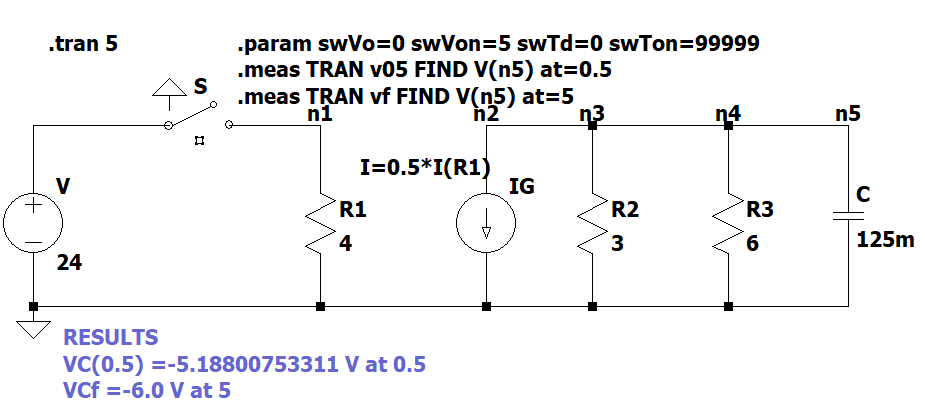
\includegraphics[width=0.8\columnwidth]{../2-3.png}
\end{figure}

\begin{wrapfigure}{r}{0.6\textwidth}
\centering
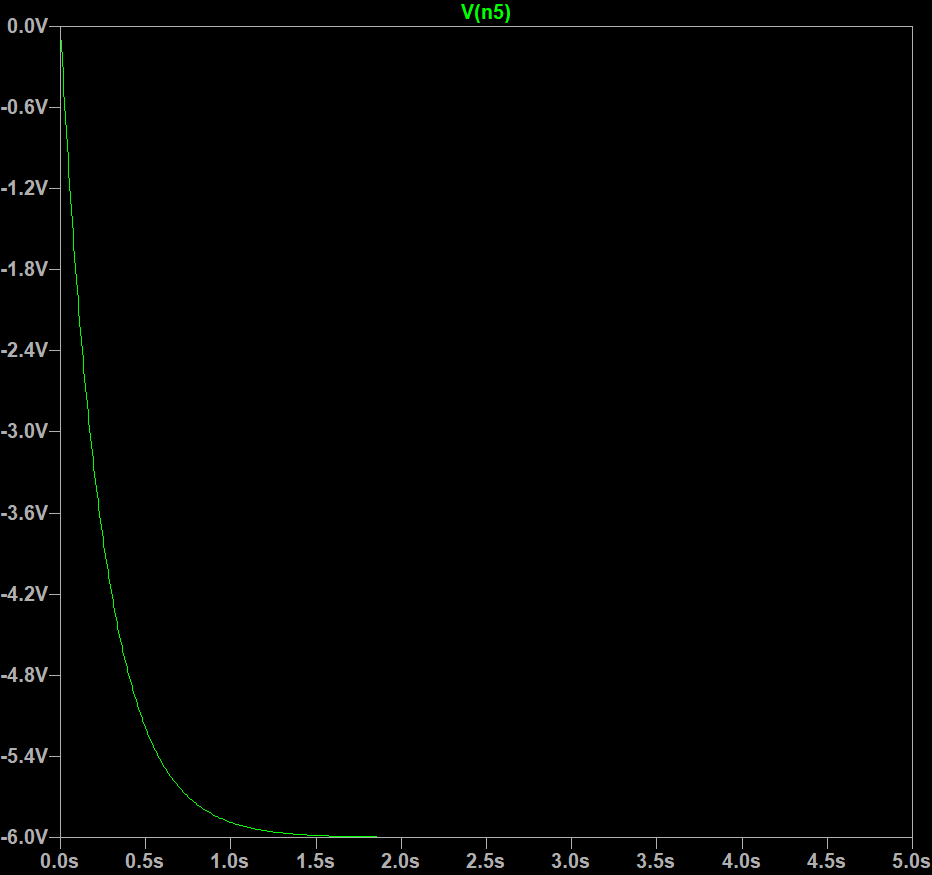
\includegraphics[width=0.8\columnwidth]{../2-3g.png}
\end{wrapfigure}

En este circuito hay una fuente de corriente dependiente del voltaje de otra resistencia tal que $I_G=0.5I_{R1}$. La malla de la izquierda sólo sirve el propósito de proporcionar un voltaje para la intensidad de control, y no está conectada en paralelo con el resto de mallas. 

Para $t<0$, el condensador está descargado, por lo que:
\begin{gather*}
v_C(t)=A+Be^{-\frac{t}{\tau}}\xrightarrow[(A+B=0)]{} -B+Be^{-\frac{t}{R_{eq}C}}
\end{gather*}
Necesitamos saber el voltaje inicial para hallar $B$, por lo que lo podemos hallar \clearpage aplicando nudos. Para ello, necesitamos saber $I_G$, que depende de $I_{R1}$.
\begin{gather*}
	I_{R1}=\frac{24}{4}=6\, A \rightarrow I_G=\frac{6}{2}=3\, A
\end{gather*}

Tras hacer el circuito equivalente, teniendo en cuenta que para $t\rightarrow\infty$ el condensador actúa como circuito abierto, y aplicando nudos (en el nudo equivalente que correspondería al $n2$ y $n3$), podemos hallar $v_C(\infty)$:
\begin{gather*}
	R_{eq}=\frac{1}{\frac{1}{R_2}+\frac{1}{R_3}}=2\, \Omega \\
	0=3+I_Req+I_C = 3+\frac{V_n-0}{2} \Rightarrow Vn=\boxed{v_C(\infty=-6\, V)}
\end{gather*}

Sustituimos en $v_C(t)$ para hallar la expresión del voltaje con el tiempo, y posteriormente la aplicamos para $0.5\, s$:
\begin{gather*}
	\boxed{v_C(T)=-6+6e^{-4t}\, V} \; ; \; \boxed{v_C(0.5)=-5.19\, V}
\end{gather*}

\section{Práctica 3:}

\subsection{Ejercicio 1}

\begin{figure}[h]
\centering
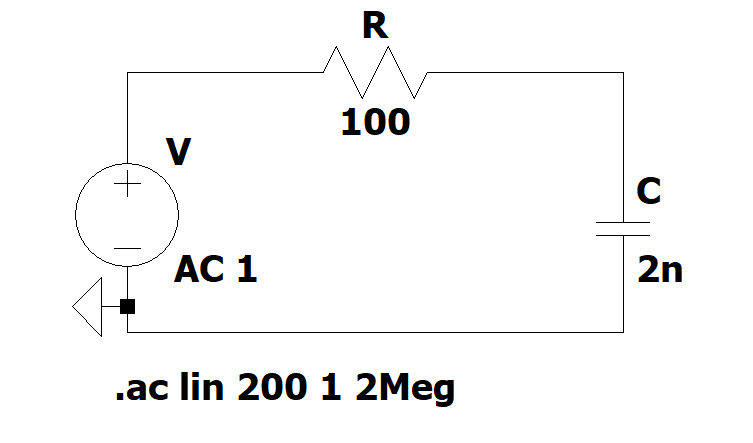
\includegraphics[width=0.5\columnwidth]{../3-1.png}
\end{figure}

\begin{wrapfigure}{r}{0.5\textwidth}
\centering
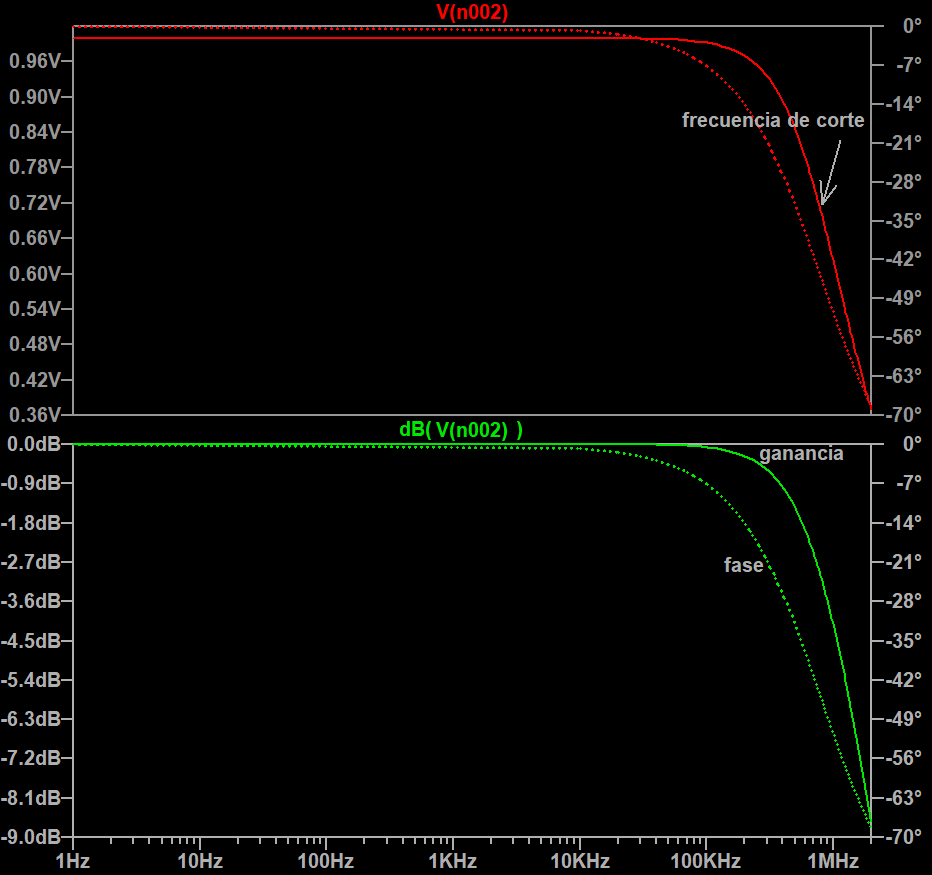
\includegraphics[width=0.95\columnwidth]{../3-1g.png}
\end{wrapfigure}

Para este circuito se ha tenido que realizar un barrido de corriente alterna, que modula la frecuencia de la misma de un valor a otro escogido y devuelve los resultados del circuito para cada frecuencia. Se ha usado un barrido lineal, para poder elegir el orden de los incrementos. Para tener un barrido con incrementos de $10\, kHz$, debemos indicar que queremos que tenga $200$ puntos, ya que $\frac{2000000-1}{10000}\approxeq 200$. Observamos que para frecuencias altas, la ganancia en decibelios es $0$, y al ser una escala logarítmica, significa que $\frac{V_{out}}{V_{in}}=1$, valor que esperamos ya que el filtro \textbf{pasa-baja} permite el paso de las frecuencias más bajas. En cambio, observamos que conforme la frecuencia va aumentando, la ganancia se vuelve más negativa, es decir, que $\frac{V_{out}}{V_{in}}$ es decimal, por lo que está siendo atenuado.

En la gráfica de $V(n002)\, / \, f$, la frecuencia de corte será aquella en la que $V_{out}=0.707V_{in}$. En este caso, como se ha elegido amplitud inicial de $1\, V$, será justo en $0.707\, V$. Gráficamente nos da un valor de frecuencia de aproximadamente $800\, Hz$, que coincide con el valor teórico calculado: $f_c=\frac{1}{2\pi RC}=795.77\, Hz$.

\subsection{Ejercicio 2}

\begin{figure}[h]
\centering
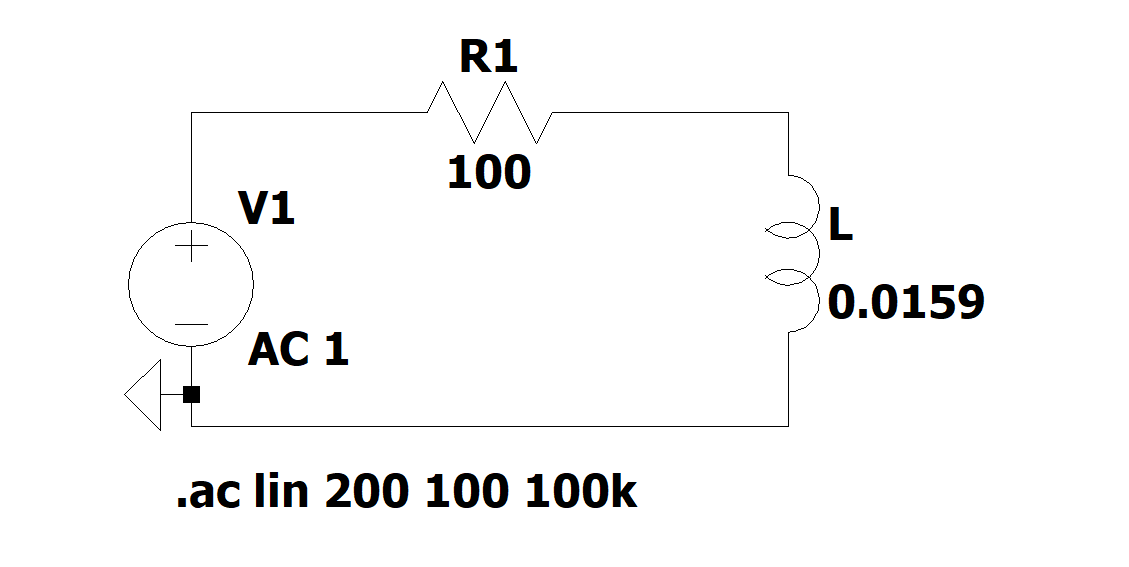
\includegraphics[width=0.6\columnwidth]{../3-2.png}
\end{figure}

\begin{wrapfigure}[10]{r}{0.5\textwidth}
\centering
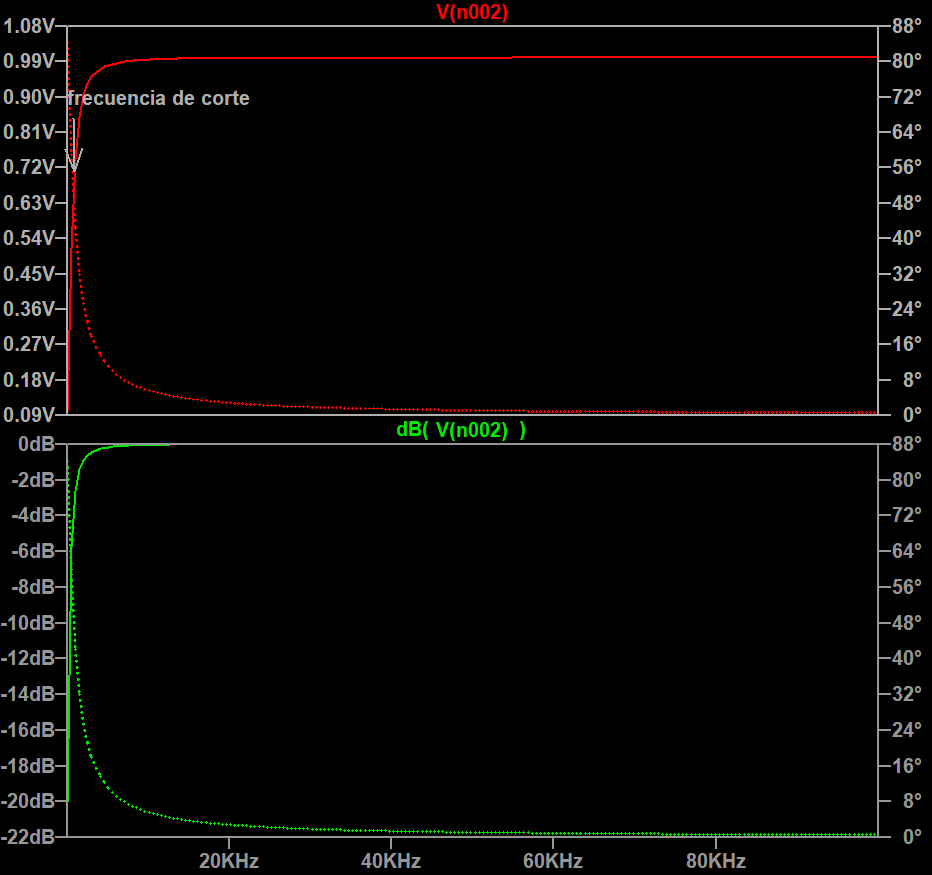
\includegraphics[width=0.95\columnwidth]{../3-2g.png}
\end{wrapfigure}

Se ha pedido que para este ejercicio la frecuencia de corte del filtro sea $f_c=\frac{R}{2\pi L}=1000\, Hz \Rightarrow L=0.0159\, H$. Tras realizar el barrido con este dato introducido, hallamos gráficamente que la frecuencia de corte es aproximadamente $1.029\, kHz$, resultado que cuadra con el enunciado del ejercicio.

Se ha realizado también el diagrama de Bode (en $dB$), representado con una traza verde, al igual que en el ejercicio anterior. 

\vspace{2.8cm}
\subsection{Ejercicio 3}

\begin{wrapfigure}[10]{r}{0.5\textwidth}
\centering
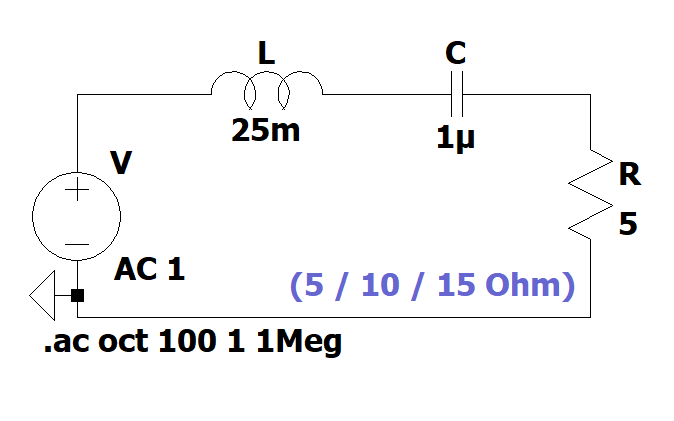
\includegraphics[width=0.95\columnwidth]{../3-3.png}
\end{wrapfigure}

Para este circuito nos piden hacer tres barridos cambiando la resistencia a $5\, \Omega,\, 50\, \Omega\, \text{ y } 100\, \Omega$. Se pueden hallar los valores teóricos de la anchura de banda, definida por: $\Delta f =f_2-f_1$, siendo éstas las frecuencias de corte correspondientes a las atenuaciones realizadas por el condensador y la bobina. Conociendo que el factor Q de un cirucito \textit{RLC} es $Q=\frac{f_o}{\Delta f}$, y sabiendo que la frecuencia de resonancia está determinada por $f_o=\frac{1}{2\pi\sqrt{LC}}$, sustituimos y despejamos:

%graphs


\begin{minipage}{.4\textwidth}
	\begin{gather*}
	f_o=\frac{1}{2\pi\sqrt{LC}} = 1006.5\, Hz\\
	Q=\frac{1}{R}\sqrt{\frac{L}{C}}\; ; \; \Delta f = \frac{f_o}{Q}
\end{gather*}
\end{minipage}
\hfill\vline\hfill
\begin{minipage}{.4\textwidth}
	\begin{table}[H]
\centering
%\def\arraystretch{1.5}
\begin{tabular}{|c||c|c|} \cline{2-3}
	\multicolumn{1}{c|}{} & \textbf{Q} & \textbf{$\Delta f$} \\ \hline
	$5\, \Omega$ & $31.62$ & $31.83\, Hz$ \\ \hline
	 $10\, \Omega$ & $15.81$ & $63.66\, Hz$ \\ \hline
	$15\, \Omega$  & $10.54$ & $95.49\, Hz$ \\ \hline
\end{tabular}
\end{table}
\vspace{2pt}
\end{minipage}
\hrule

\clearpage

\begin{wrapfigure}{r}{0.4\textwidth}
\centering
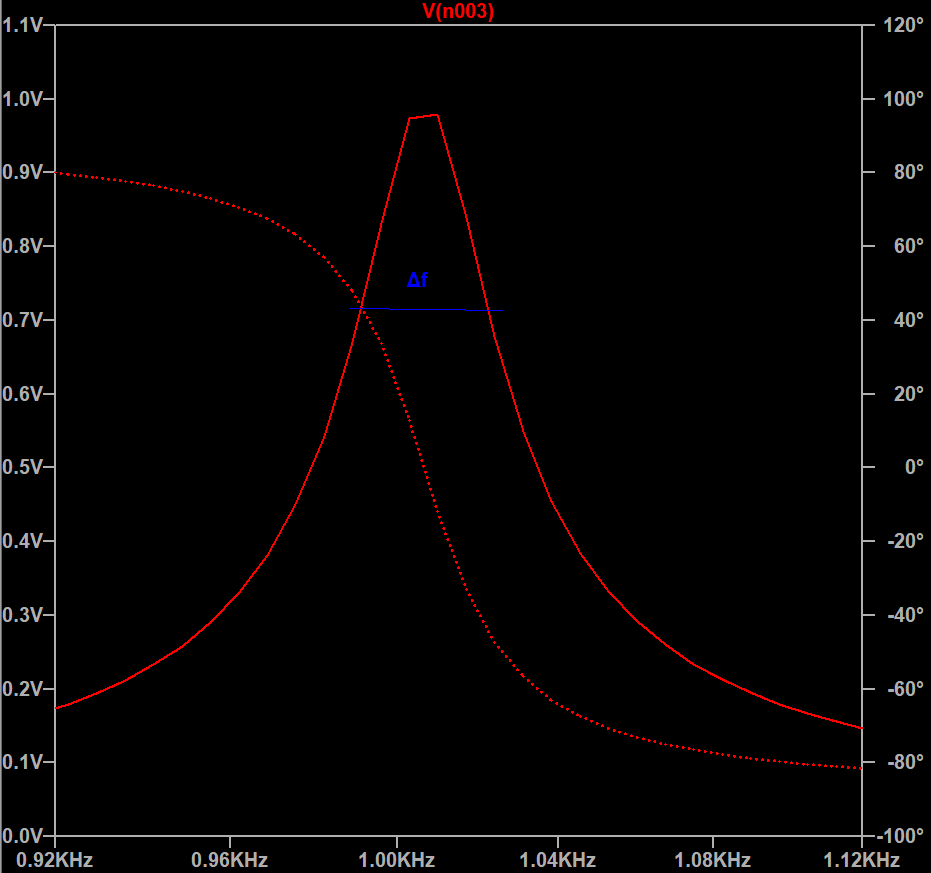
\includegraphics[width=0.95\columnwidth]{../3-med.png}
\end{wrapfigure}

Comparando los resultados teóricos con los hallados gráficamente, podemos observar que la frecuencia de resonancia coincide, siendo esta $\approx 1 kHz$. El ancho de banda lo medimos con la diferencia de las dos frecuencias de corte (en $V\approx 0.707\, V$) correspondientes a las atenuaciones por cada lado, y en todos los casos también coinciden con los teóricos. Ha sido necesario hacer zoom en la gráfica para poder apreciarlo, como se indica en el ejemplo de la derecha.

A continuación se muestran las gráficas para cada resistencia ordenadas por columnas. Dentro de cada columna, la traza roja representa el voltage frente a la frecuencia, mientras que la verde es el diagrama de Bode (\textit{hacer zoom en el PDF para ver con mayor resolución}):

\begin{figure}[h!]
	\centering
	\begin{minipage}{.32\textwidth}
	  \centering
	  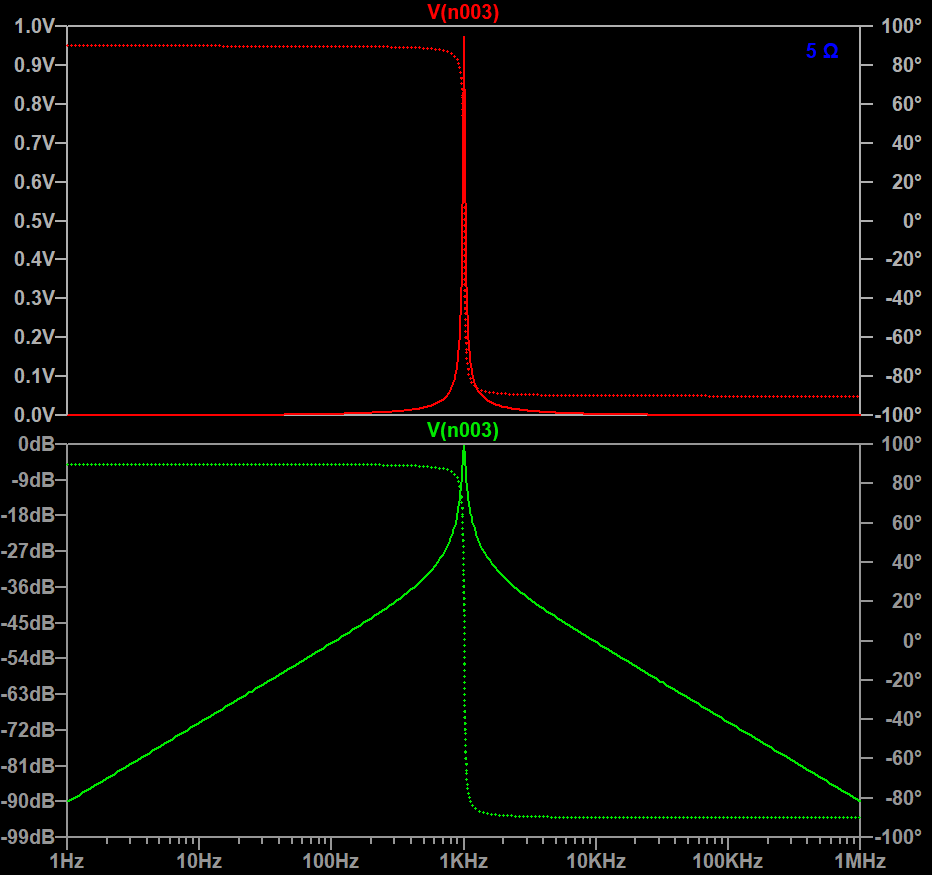
\includegraphics[width=\linewidth]{../3-35.png}
	\end{minipage}
	\begin{minipage}{.32\textwidth}
	  \centering
	  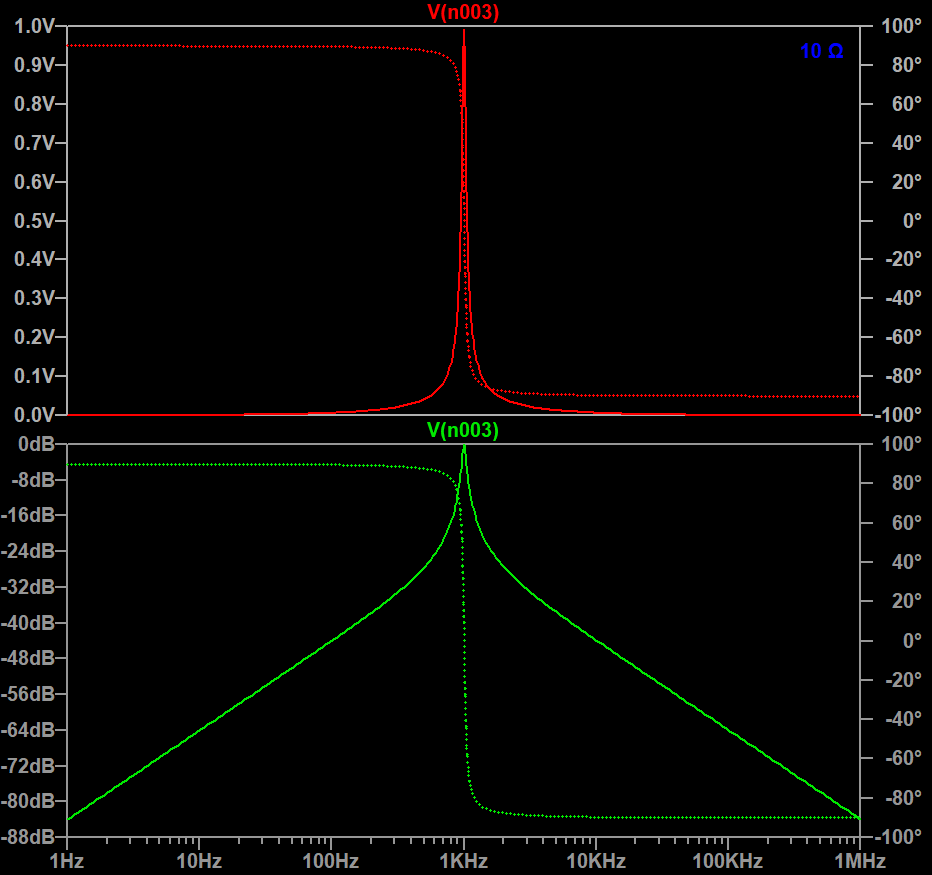
\includegraphics[width=\linewidth]{../3-310.png}
	\end{minipage}
	\begin{minipage}{.32\textwidth}
	  \centering
	  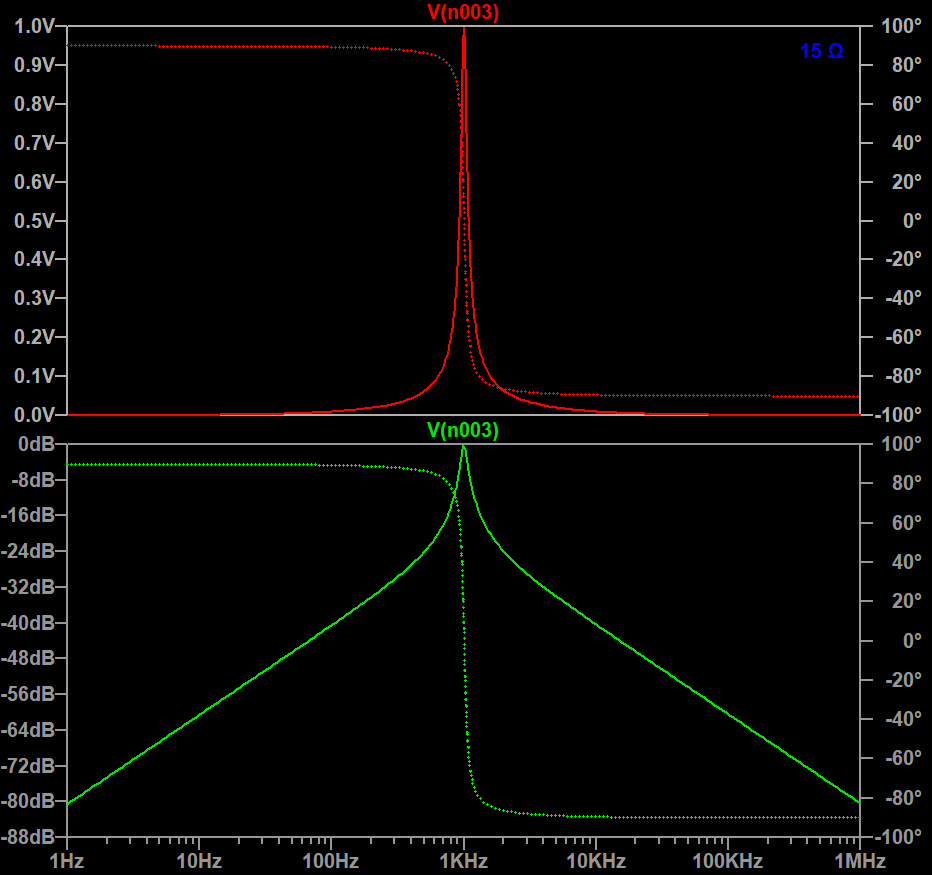
\includegraphics[width=\linewidth]{../3-315.png}
	\end{minipage}
	\end{figure}

% _________________________________________

\vspace{1.5cm}
\appendix
\label{appendix}
\textbf{APPENDIX}

\begin{figure}[h]
\centering
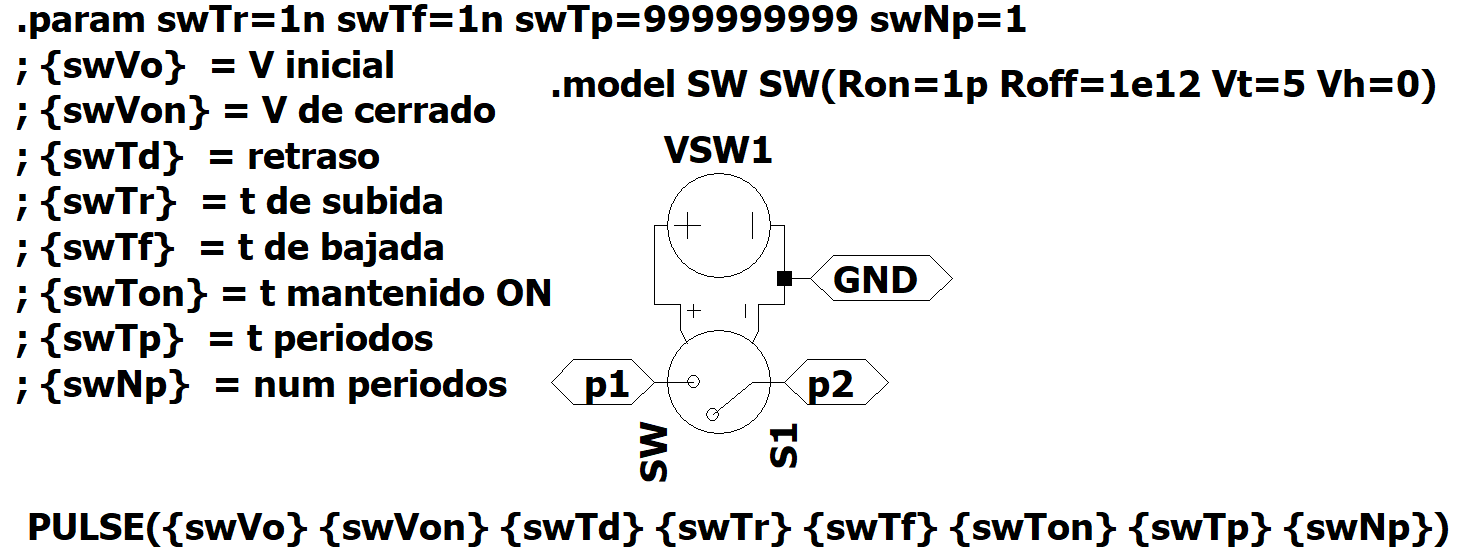
\includegraphics[width=0.7\columnwidth]{../sw.png}
\label{fig:sw}
\caption{Subcircuito de un interruptor controlado por tensión diseñado para que actúe como un interruptor que se pueda abrir o cerrar en los intervalos de tiempo deseados. Tiene un pin a tierra, ya que es conveniente no usar tierras internas en subcircuitos en LTspice.}
\end{figure}

\vspace{2cm}
\begin{center}
\setlength{\fboxsep}{0.5cm}
\shadowbox{\begin{minipage}{10.5cm}
\textbf{Declaración de Autoría}\\

El alumno
Álvaro Jerónimo Sánchez
, con DNI número 
09847051S
, declara que es el autor único e individual de este trabajo.\\

\vspace{3cm}
Fdo:

\end{minipage}}
\end{center}

\end{document}